\begin{qu}[Filter for an antenna]\num
The capacitor is used to filter out DC and low frequencies coming from the voltage
source, so that only radio-frequency signals get to the transmitting antenna.

\vspace{5mm}

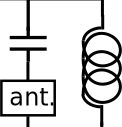
\includegraphics{electromagnetism/figs/antenna-filter}

\vspace{5mm}

\noindent Suppose we add the inductor as shown. What is the effect on the signal
\emph{felt by the antenna?}

A. There is no effect.

B. The coil is not needed for DC, but improves filtering of low frequencies.

C. The filtering gets worse because we're adding a big impedance at high
frequencies.

D. The filter now acts as a bandpass filter centered on $\omega=(LC)^{-1/2}$.

\end{qu}
